%% ma: L12-B02-0014
%% lop: 12
%% chuong: 1
%% bai: 2
%% dang: 12.2.10
%% loai: TN4
%% muc: TH
%% dap_an: "C"
%% nguon: "HK1-DeOn_1_1.pdf (M10, Đề ôn tập học kì 1 Toán 12, Đề số 2), Phần I Câu 9"
%% kien_thuc: "Bài 1 (tính đơn điệu và cực trị), Bài 2 (giá trị lớn nhất, nhỏ nhất)"
%% trang_thai: chinh-thuc
%% ghi_chu: "Đã duyệt 29/10/2026."
\begin{ex}
Cho hàm số $y=\dfrac{2x+8}{x+2}$ có bảng biến thiên như hình vẽ:
\begin{center}\begin{tikzpicture}
\tkzTabInit[lgt=1.2,espcl=3]{$x$/.8,$y'$/.8,$y$/2.2}{$-\infty$,$-2$,$+\infty$}
\tkzTabLine{,-,d,-,}
\tkzTabVar{+/$2$,-D+/$-\infty$/$+\infty$,-/$2$}
\end{tikzpicture}\end{center}
Giá trị lớn nhất của hàm số trên đoạn $[0;1]$ là
\choice{$8$}{$10$}{\True $4$}{$2$}
\loigiai{Hàm số nghịch biến trên $(-2;+\infty)\supset[0;1]$ nên $\max\limits_{[0;1]}y=y(0)=4$.}
\end{ex}
